\chapter{Background}
\label{chap:background}

In this chapter, I will discuss some of the background relevant to the task at
hand, including a short overview of word-sense disambiguation broadly, its
history with respect to machine translation, and how the cross-lingual framing
of WSD addresses some of the difficulties in successfully applying WSD
techniques to MT. I also give a short description of the languages we aim to
support with this work, Guarani and Quechua.

\section{Word-Sense Disambiguation}
Word types often -- or perhaps always, to take a philosophical view of 
communication and semiosis -- have many possible meanings. Given a string of
characters or an utterance, the reader or listener must do some computational
work to interpret the received message, and this may fail.
In the simplest case, one could be faced with
a homophone or homograph and need to distinguish between different lexemes that
could be intended. There could be technical or jargon senses that conflict with
colloquial uses of a word; consider the many different meanings of ``kernel",
``type" and ``kind" in computer science and mathematics. In the most difficult
case, the usages can be hyperbolic, metaphorical, sarcastic, or oblique
references. Understanding these usages will require understanding the broader
discourse context and the goals of the speaker. Discourse modeling is outside
the scope of this work, but in practice, for machine translation, we will need
to get some sense of the particular meaning of a polysemous word, in context.

What we mean by word sense disambiguation is just this:
when faced with a token in a piece of text, we want to be able to
decide which \emph{word sense} from a \emph{sense inventory} is the intended
meaning. The sense inventory might come from a pre-set ontology built by
lexicographers, such as a
dictionary or a WordNet, or it might have  been discovered in some automatic
way. Word-sense disambiguation tasks have typically been divided into two
varieties, where \emph{lexical sample} tasks require labeling occurrences of
some small number of words types, and \emph{all-words} tasks, in which every
word in the input text must be labeled. In NLP applications faced with
arbitrary text, this distinction may not be relevant, as the application will
encounter previously unseen words, for which there are no known senses in the
ontology.

When making use of WSD for some other purpose -- say in information retrieval,
information extraction, or machine translation -- choosing an appropriate sense
inventory can be a difficult design task, as applications may require different
granularities, while different lexicographers will have made their own
editorial decisions about what constitutes a distinct sense of a word.

\begin{figure}
  %% XXX
  OMFG THERE ARE SO MANY SENSES
  \caption{WordNet 3.1 senses for the verb ``take". In WordNet and similar
  projects, word senses are called \emph{synsets}, as there will be a set of
  synonyms that share the sense.}
  \label{fig:wordnet-senses-take}
\end{figure}

Treating WSD as a supervised learning problem requires labeled training data,
which for this task means text where each token has been annotated with its
appropriate sense identifier. 
Such corpora must be created manually specifically for this purpose, and this kind
of annotation is very labor-intensive, especially when annotating data for an
all-words WSD task, as the annotators must consider the many possible senses
for each word, and new words will occur during the course of annotation.

%% XXX look up and get reference for ... line hard serve corpus ...
Sense-annotated corpora have been created for supervised WSD for both the lexical
selection and all-words settings, but they are only available for a few
languages, due to the time and effort required to prepare them.
Some famous sense-annotated corpora include the hard/line/serve corpus, which
marked hard/line/serve with their respective senses from WordNet (XXX check
this). It features XXX sentences, each manually annotated, and it was used for
the XXX SensEval shared task.
There have also been all-words annotated corpora, such as the MASC and
SemCor corpora, which included XXX sentences annotated with their WordNet
senses... (XXX cite these too).

In order to ameliorate this WSD data acquisition bottleneck and allow WSD
research to move forward in the absence of annotated training data, researchers
have also created corpora with artificially-ambiguous ``pseudo-words". Ted
Pedersen, for example, provides scripts to automatically conflate two common
words by replacing them both with the same token\footnote{Available at
\url{XXX the website}}. The original uses are then considered two senses of the
new pseudo-word, and researchers can check whether their WSD algorithms can
recover the original token.

For a broad overview of the history of and different approaches to word sense
disambiguation, please see Agirre \emph{et al.}'s book on the topic.
\cite{agirre2006word}
Supervised-learning approaches are by no means the only strand of research;
there are also unsupervised word-sense induction approaches,
knowledge-based heuristics that make use of hand-crafted resources such as
dictionaries...
%% XXX

It has long been held that word sense disambiguation is a central problem in
NLP applications, including machine translation.
Even in popular culture, the dangers of misunderstanding and thus
mistranslating individual words is well-understood; many have heard the
(apparently apocryphal \cite{hutchins:whiskey}) story about an early MT system
faced with the Biblical saying ``the spirit is willing but the flesh is
weak" in Russian and producing (variations on the story abound) ``the vodka is
good but the meat is rotten".

As early as 1960, Yehoshua Bar-Hillel wrote that general-purpose machine
translation (``fully automatic high-quality  translation", as it was  called at
the  time) was impossible due to the insurmountable task of writing WSD
routines for all source-language words. \cite{barhillel1960}

\begin{quote}
During the past year I have repeatedly tried to point out the illusory
character of the FAHQT ideal even in respect to the mechanical determination of
the syntactical structure of a given source-language sentence... Here I shall
show that there exist extremely simple sentences in English -- and the same
holds, I am sure, for any other natural language -- which within certain
linguistic contexts, would be uniquely (up to plain synonymy) and unambiguously
translated into any other language by anyone with a sufficient knowledge of the
two languages involved, though I know of no program that would enable a machine
to come up with this unique rendering unless by a completely arbitrary and
\emph{ad hoc} procedure whose futility would show itself in the next example.

A sentence of this kind is the following: \emph{The box was in the pen.}
\end{quote}

To produce a correct rendering of this sentence in Spanish, for example, the
translation system must decide between translating ``pen" as \emph{corral} (an
enclosure, like for an animal) or as \emph{pluma} (the instrument for writing).

As of this writing, for this particular example, Google Translate picks the
correct rendering, although in September 2013, it chose the less-sensible 
``in the writing implement" translation (see Figure \ref{fig:box-in-pen}).

One wonders how this could have come about -- we would hope that the n-gram
language model for Spanish would prefer sentences about things in enclosures to
things in writing implements.
But the word \emph{en} can be a translation of either the English ``in" or
``on", and \emph{pluma} can also mean ``feather", so \emph{en la pluma} will be
attested in a large corpus of Spanish; we could easily imagine a sentence
containing ``on the feather". This situation is fairly complex.

\begin{figure}
  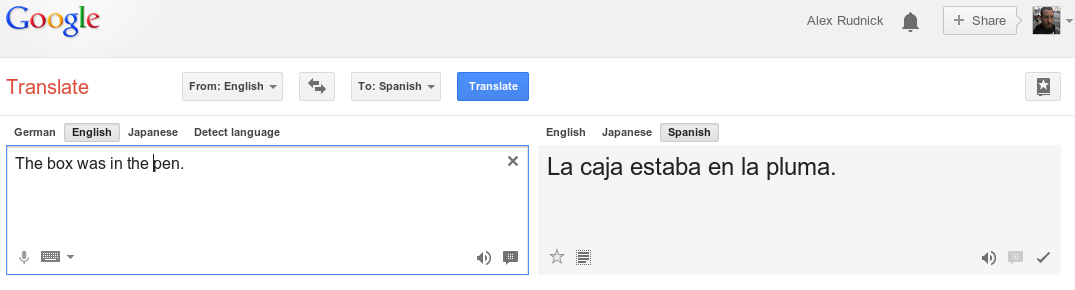
\includegraphics[width=12cm]{box-in-pen.png}
  \caption{Google Translate, September 17, 2013; interestingly, adding or
  removing the final period in the English sentence caused a switch between the
  ``pluma" and ``corral" renderings.}
  \label{fig:box-in-pen}
\end{figure}

In a translation task, even if we are able to assign a particular sense to a
given word, we must still map these senses to translations in the target
language, and there is no guarantee that senses identified by source-language
lexicographers will map neatly to distinctions made by the target language.

%% XXX: "serious rain" in Russian, "cut/break" verbs that depend on different
%% distinctions...

%% XXX: light verbs...


\section{Cross-lingual word sense disambiguation}
\label{sec:clwsd}

This problem that Bar-Hillel identified as difficult, the one that arises
in the apocryphal ``spirit is willing" story, is a particular variant of word
sense disambiguation that we here call \emph{cross-lingual WSD} (CL-WSD).
In a CL-WSD task, we  want to label words or phrases in the input text with
their contextually-appropriate translations in some target language. Here the
sense inventory for each word is defined as its possible translations.
Typically, the possible translations are discovered automatically from a
word-aligned bitext corpus, although a dictionary or other bilingual lexicon
may also be used as source of possible translations.

This setting for WSD has immediate applications in machine translation. It
also neatly addresses the problem of choosing an appropriate sense inventory,
which has historically been a difficult problem for the practical application
of WSD systems \cite{agirre2006word}: the sense distinctions that the system
should learn are exactly those that are lexicalized in the target language.
CL-WSD also sidesteps the ``knowledge acquisition bottleneck" hampering other
work in WSD \cite{lefever-hoste-decock:2011:ACL-HLT2011}.
While supervised CL-WSD methods typically require bitext for training, this is
more readily available than the sense-annotated text that would otherwise be
required.

WSD applied directly to machine translation has a long history; practical work
in integrating WSD with statistical machine translation particularly dates back
to early SMT work at IBM \cite{Brown91word-sensedisambiguation}, but the
problem itself was described in Warren Weaver's prescient 1949 memorandum
\cite{weavermemo}, which describes an essentially modern conception of WSD.

This cross-lingual variant of WSD has received enough attention to warrant
shared tasks at recent SemEval workshops: SemEval 2010 Task 3
\cite{lefever-hoste:2010:SemEval} and SemEval 2013 Task 10 \cite{task10} were both
explicitly about CL-WSD.  A similar task was also run in 2014
\cite{vangompel-EtAl:2014:SemEval}, although this task provides a
target-language context rather than a source-language one, more closely
representing the problem faced by an agent trying to help a second-language
learner compose a sentence in their L2 than that faced by a machine translation
system. Some approaches to the first two tasks, along with a number of other
projects, are described in Chapter~\ref{chap:relatedwork}.

In general, there is a many-to-many relationship across language boundaries
between words and their possible translations.
This happens for a number of reasons: figurative or metaphorical uses may not
translate directly,
obligatory information in one language may be left unspecified in another,
or the criteria for selecting a word may simply differ.
To give some familiar examples, a ``leg" of a trip in English is typically
translated as \emph{etape} in French, which is unrelated to limbs used for
walking;
translating ``brother" to Japanese requires specifying whether the brother is
older (\emph{ani}) or younger (\emph{ot\=oto});
a soap bubble or a ceramic plate can be destroyed with the same word in
Chinese, whereas English speakers distinguish between the verbs
``pop" and ``break" \cite{majid2007semantic}.

Despite these difficulties, most statistical MT systems do not use an explicit
WSD module \cite{wsdchap3}; the language model and phrase tables of these
systems mitigate lexical ambiguities by encouraging words used collocationally
to appear together in the output. Entire phrases\footnote{Not necessarily
``phrases" in a syntactic sense, but subsequences of sentences} such as verbs
with their common objects may be learned and stored in the phrase table, and
the language model will encourage common collocations as well.

To take a look at some apparently easier examples, let us also consider the
following usages of \emph{letter}, from the test set of a recent SemEval shared
task \cite{task10}, and how to translate them into Spanish.

\enumsentence{
But a quick look at today's \emph{letters} to the editor in the Times suggest
that here at least is one department of the paper that could use a little more
fact-checking. }
\label{sent:carta}
\enumsentence{
All over the ice were little Cohens, little Levys, their names sewed in block
\emph{letters} on the backs of their jerseys. }
\label{sent:letra}

We would want (\ref{sent:carta}) to be translated with the word \emph{carta},
and (\ref{sent:letra}) to be translated with \emph{letra} or something similar.
Google Translate (as of this writing) handles both of these sentences well,
rendering the first with ``cartas" and the second with an even better choice,
translating the phrase ``block letters" as \emph{mayúsculas}.
However longer-distance relationships, search errors, or simple statistical
accidents can still cause strange translations in practice.

\begin{figure}
  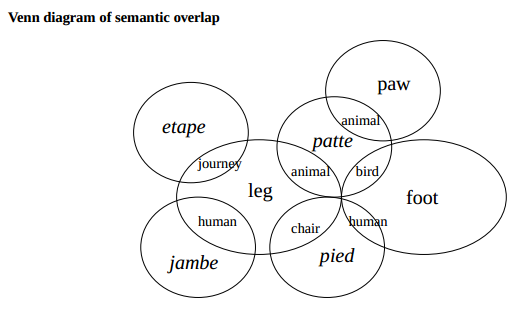
\includegraphics[width=12cm]{hutchins-leg-etc.png}
  \caption{Overlap of words related to ``leg"; relationships between English
  and French words. Figure 21.2 from \protect\cite{slp1}; example originally
  from \protect\cite[Chapter 6]{hutchins1992introduction}.}
  \label{fig:leg}
\end{figure}


\section{Hybrid MT}
Recently there has been renewed interest in machine translation systems that
take into account syntactic structure, linguistic knowledge, and semantic
representations, perhaps due to a perception that statistical approaches
relying on flatter phrase-based representations and hierarchical
representations not based on linguistic intuitions are reaching a performance
%% plateau.
%% , such as the classical
%% phrase-based SMT XXX cite Koehn et al, and nested representations learned
%% without regard to linguistic intuitions...

The boundaries between rule-based and statistical MT systems are becoming
increasingly blurred, and hybrid systems are being developed in both
directions, with RBMT systems incorporating components based on machine
learning, as well as SMT systems making use of linguistic knowledge for
morphology and syntax.
Rule-based components are especially applicable in cases where the language
pair involves predictable reordering through syntactic divergences
(XXX citation)
and in cases where one or both sides of the translation pair exhibits rich
morphology; morphological analysis and generation software generally consists
of hand-written rules in the form of finite-state transducers.

Additionally, for most of the world's language pairs, there is simply no large
bitext corpus available, so training a purely statistical machine translation
system is infeasible.\footnote{Techniques for learning from comparable corpora,
such as translation spotting, are under development, and there has been some
work on building sufficiently large bitext corpora through crowdsourcing, but
these approaches have not yet reached wide adoption.}
As such, RBMT approaches are still relevant for many language pairs, and there
is a vibrant research community focused on building linguistically-informed
primarily rule-based machine translation systems.

We would like for RBMT or hybrid systems, once developed, to be able to make
use of any bitext resources that are available, or that become available later.
Like SMT systems, they should be able to produce better translations as larger
corpora are developed, without additional code changes: this is the main
engineering goal for the Chipa software.

\urldef{\leydelenguas}\url{http://www.cultura.gov.py/lang/es-es/2011/05/ley-de-lenguas-n%C2%BA-4251/}

\section{Paraguay and the Guarani Language}
Guarani is an indigenous language spoken in Paraguay and the surrounding
region.
Historically, it was the native language of the indigenous Guarani people. The
word for the Guarani language in Guarani is \emph{avañe'e} (``people's
language", where \emph{ñe'e} means ``language").

Guarani is unique among indigenous American languages in that a substantial
number of non-indigenous people speak it.  The majority of Paraguayans are
conversant in Guarani, although they are likely to be bilingual with Spanish.
In practice, many Paraguayans use a combination of Guarani and Spanish called
\emph{Jopar{\'a}}, which is the Guarani word for ``mixture".

Paraguay is officially a bilingual, pluricultural country, as described by its
famous \emph{Ley de Lenguas} \footnote{\leydelenguas} (``Law of Languages").
However, the Guarani language is at a significant social and economic
disadvantage and is typically not used in formal situations, as Spanish is
considered more prestigious. There are, however, an engaged activist
community, many Guarani-language educators, and a government agency devoted
specifically to policy regarding language.
The Guarani language figures significantly into a sense of Paraguayan national
identity and history.

Guarani has a rich, polysynthetic, agglutinative morphology, in which roots can
derive into different parts of speech, and often several roots can combine into
a single word. Guarani morphology can mark tense, aspect (even on nouns),
number, negation, and other features. However, unlike Spanish, it has no
grammatical gender.  Guarani's rich morphology can make many NLP tasks,
including ones seemingly as simple as spell-checking, rather challenging.

We are in contact with a number of collaborators in Paraguay, including
language activists and educators from the \emph{Ateneo de la Lengua y Cultura
Guaraní} \footnote{\url{http://www.ateneoguarani.edu.py/}} and the
\emph{Fundación Yvy Marãe'{\~y}} \footnote{\url{http://yvymaraey.org/}},
both of which are schools that offer training for Guarani-language translators.
We have also been discussing development plans with several local software
developers, including members of the local One Laptop Per Child organization
and the Secretariat of Language Policies.
%% XXX mention Guampa?

\subsection{Online Language Tools for Guarani}
There are currently very few online language tools for Guarani; some of the
best available ones are iGuarani \footnote{\url{http://iguarani.com/}}, a
searchable online dictionary and gisting translation system developed by young
Paraguayan programmer Diego Alejandro Gavilán.

There is also a small searchable online dictionary developed by Wolf Lustig
\footnote{\url{http://www.uni-mainz.de/cgi-bin/guarani2/dictionary.pl}},
which has versions in Spanish, German, and English. He has graciously made this
dictionary available for our use, and this will provide a starting point for
our Spanish-Guarani translation system.

The Guarani activist and education community has a presence on the Web,
although a startlingly large fraction of this presence is a single author,
Dr. David Galeano Olivera, the president of the \emph{Ateneo de Lengua y
Cultura Guaraní}. He has collected a number of resources, written in Spanish
and Guarani, about the Guarani language and the culture surrounding it.
\footnote{\url{http://cafehistoria.ning.com/profiles/blogs/la-lengua-guarani-o-avanee-en}}
